\section*{Task 2 --- Leaderboard Challenge}

\subsection*{2.1 What the data says}
\begin{itemize}
\item \textbf{Sampling and horizon.} 43,824 rows is $5\times8{,}760$, so the series is almost certainly hourly over five years, and the horizon of 168 steps is one week. The mean by index mod 24 shows a clear daily cycle (Fig.~T2-1).
\item \textbf{Memory is short.} The autocorrelation is 0.97 at lag 1, 0.40 at lag 24, 0.16 at lag 48 and 0.03 at lag 168. The past alone says little about the second half of the week.
\item \textbf{Heavy tail.} Mean 98, median 73, 99th percentile 418, maximum 994. RMSE is dominated by the rare high episodes.
\item \textbf{The optional file is future-known weather.} It has 6 continuous and 4 mutually exclusive binary columns: two temperature-like columns (A, B), pressure (C), a cumulative wind speed that restarts when the binary state changes (D), and two rare cumulative counts (E, F). The four flags behave like a wind-direction indicator. The target mean under each flag is G 90, H 70, I 110, J 125: flag H clears the air, while J (stagnant conditions) lets it accumulate.
\end{itemize}
\begin{figure}[H]\centering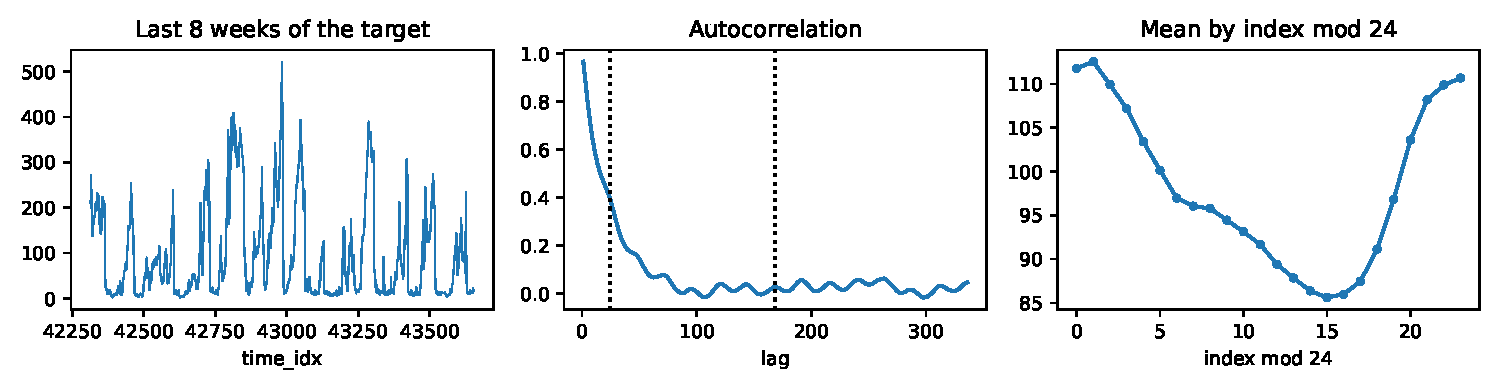
\includegraphics[width=\linewidth]{../Figures/T2-1_data.pdf}\caption*{Fig.~T2-1 --- last 8 weeks, autocorrelation, daily profile.}\end{figure}

\subsection*{2.2 Validation protocol (fixed before any v3 study)}
With 5 leaderboard attempts, the leaderboard cannot be a tuning signal, so every decision below uses my own chronological validation.
\begin{itemize}
\item \textbf{Two folds}, each trained only on rows before it:
  \begin{itemize}
  \item \emph{winter}: rows 33,600--36,480. If the series starts on 1 January, this is November--February of the previous winter. The hidden week is then the last week of December, so this fold matches its season.
  \item \emph{recent}: the last 16 weeks of the history.
  \end{itemize}
\item \textbf{Scoring.} A forecast starts every 24 steps, giving 220 forecasts of 168 steps in total. All lead times are scored on the raw scale with RMSE, MAE and sMAPE.
\item \textbf{Seeds.} Every option is trained with 3 seeds. I report the per-seed mean $\pm$ std and the RMSE of the 3-seed average.
\item \textbf{Selection rule.} The option with the lowest mean per-seed RMSE, pooled over both folds, wins.
\end{itemize}
\emph{Why two folds?} A single 168-step validation block is noisy: the gap between two designs can be smaller than week-to-week variation, so one block is a weak basis for model selection.

\subsection*{2.3 Model: an encoder--decoder Autoformer}
I wrote the model from scratch, following Wu et al.\ (2021), \S\S3.1--3.2, and reusing my own Task 1 decomposition and delay-aggregation code. It contains both required mechanisms:
\begin{itemize}
\item \textbf{Series decomposition (progressive).} A moving average (kernel 25, endpoint replication) splits the input into seasonal and trend parts. The same split is applied again after \emph{every} sub-layer of the encoder and decoder. The trend pieces removed in the decoder are projected and accumulated into the trend path.
\item \textbf{Auto-Correlation.}
  \begin{itemize}
  \item Delay scores $R(\tau)=\sum_t q_t k_{t-\tau}$ are computed by FFT in $O(L\log L)$, and the top $k=\lfloor 2\ln L\rfloor$ delays are kept: $k=9$ in the encoder ($L=96$) and $k=10$ in the decoder ($L=48+168=216$).
  \item Weights: $\alpha=\mathrm{softmax}(R/\vartheta)$ with a learned temperature $\vartheta$.
  \item Aggregation: $z_t=\sum_j \alpha_j v_{t-\tau_j}$.
  \item The decoder uses it twice: on itself, and across to the encoder output.
  \item There is no dot-product attention anywhere in the model.
  \end{itemize}
\item \textbf{Lengths and size.}
  \begin{itemize}
  \item Context $L=96$ (memory is short, \S2.1); decoder input = last 48 context steps + 168 placeholder steps; \texttt{pred\_len}$=168$.
  \item $d_{model}=16$, one encoder layer, one decoder layer: 9,159 parameters.
  \end{itemize}
\item \textbf{Normalisation.} Global standardisation of the raw target, fitted on the training rows only. I did not use window-relative normalisation, because the absolute level is what the weather explains.
\end{itemize}
\emph{Two design changes of my own:}
\begin{enumerate}
\item \textbf{Covariate embedding.} Covariates enter through a 2-layer MLP followed by a centred depthwise temporal convolution (kernel 5), so each step also sees the weather of nearby hours. This was not ablated on its own; it is part of every covariate row in S1.
\item \textbf{Trend start.} The decoder trend starts at the context mean \emph{plus a linear function of the covariates}, instead of the paper's context mean alone. Over a whole week the level is set by the weather, not by the past window. This is tested in S2.
\end{enumerate}

\subsection*{2.4 Where the optional data enters, and what it did}
The covariates for the horizon are known at forecast time, so they enter the \textbf{decoder} at all 168 forecast steps. Past covariates enter the encoder.

\textbf{Engineered features} (all backward-looking, scaled on training rows only):
\begin{itemize}
\item hourly wind speed, recovered from the cumulative column D (it restarts when the direction flag changes);
\item that wind speed split by direction flag, each smoothed with an exponential moving average with half-lives of 6, 24 and 72 h (pollution builds up and is flushed out gradually);
\item the A$-$B gap (dew-point-depression style humidity proxy), the share of flag-J (calm) hours, and the 24-h change in C;
\item sin/cos of the daily (24) and yearly (8,766) position, to recover the cycles without timestamps.
\end{itemize}
This gives 34 inputs per step. The four index-derived sin/cos terms do not come from the optional file, so they are kept in every S1 row, including ``none''.

\begin{table}[H]\centering\small
\caption*{Study S1 --- ablation of the optional file (final architecture, 3 seeds, both folds)}
\begin{tabular}{lccccc}\toprule
Optional data & RMSE / seed & 3-seed avg & winter & recent & MAE / sMAPE\\\midrule
none & 142.6 $\pm$ 3.7 & 141.9 & 142.6 & 141.1 & 120.6 / 95.0\%\\
raw file, past only (horizon masked) & 125.9 $\pm$ 0.5 & 124.7 & 127.7 & 121.3 & 104.4 / 90.2\%\\
raw file, past + future & 85.9 $\pm$ 11.1 & 81.0 & 81.1 & 80.9 & 62.4 / 68.6\%\\
\textbf{engineered, past + future} & \textbf{81.8 $\pm$ 9.8} & \textbf{76.8} & 75.8 & 77.8 & 59.3 / 66.2\%\\\bottomrule
\end{tabular}\end{table}
\begin{figure}[H]\centering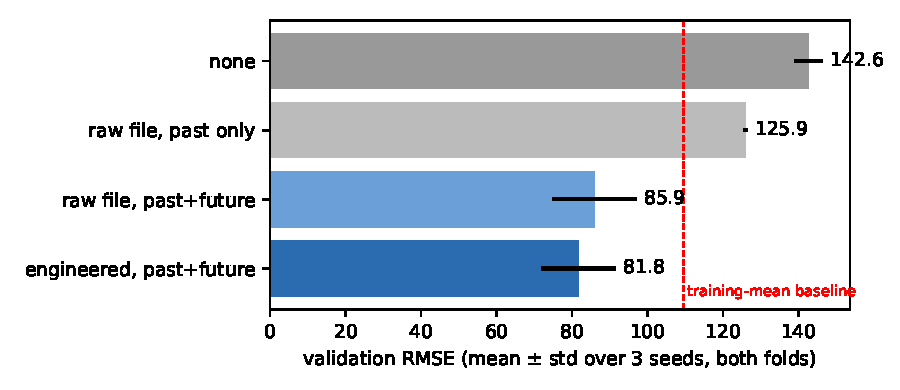
\includegraphics[width=0.6\linewidth]{../Figures/T2-2_ablation.pdf}\caption*{Fig.~T2-2 --- S1 ablation; dashed line = training-mean baseline.}\end{figure}
\textbf{Finding.} The optional file helps a lot, but only its \emph{horizon} part does: past-only covariates help a little (142.6 $\to$ 125.9), while adding the horizon covariates cuts the error by a further 32\% (125.9 $\to$ 85.9). The engineered features then gain another 4.1 (85.9 $\to$ 81.8). Both target-only and past-only models are worse than the training-mean baseline (116.3 / 102.8 on the two folds). Without future weather, the short memory leaves nothing to predict a week ahead, and the model fits noise.

\subsection*{2.5 Design studies (each starts from the winner of the previous one)}
\begin{table}[H]\centering\small
\begin{tabular}{llccc}\toprule
Study & Option & RMSE / seed & 3-seed avg & chosen\\\midrule
S2 trend start & context mean (paper) & 83.9 $\pm$ 3.1 & 80.7 & \\
 & mean + linear(covariates) & 81.8 $\pm$ 9.8 & 76.8 & \checkmark\\\midrule
S3 target & raw & 81.8 $\pm$ 9.8 & 76.8 & \checkmark\\
 & log1p & 163.2 $\pm$ 72.6 & 128.5 & \\
 & average of raw and log models & 107.2 $\pm$ 37.7 & 93.3 & \\\midrule
S4/S5 epochs & 1 & 77.8 $\pm$ 0.3 & 75.4 & \\
 & 2 & \textbf{77.1 $\pm$ 1.0} & \textbf{74.0} & \checkmark\\
 & 3 / 4 / 6 & 82.7 / 81.8 / 89.3 & 79.5 / 76.8 / 86.0 & \\\midrule
S6 width & $d=8$ / 16 / 32 & 77.2 / \textbf{77.1} / 81.7 & 72.9 / 74.0 / 72.2 & $d=16$\\\midrule
S7 dropout & 0.1 / 0.3 & \textbf{77.1} / 88.9 & 74.0 / 73.2 & 0.1\\\bottomrule
\end{tabular}\end{table}
\begin{itemize}
\item \textbf{Trend start.} The covariate trend wins on the mean (81.8 vs 83.9), and by 4 points in the 3-seed average.
\item \textbf{Target scale.} The log target is unstable: one seed exploded, because \texttt{expm1} amplifies any error at high values. The raw target matches the RMSE that is scored.
\item \textbf{Epochs.} Two epochs are best, and the model overfits beyond that (Fig.~T2-3). One epoch is the most stable ($\pm0.3$) but under-fits the winter fold (79.2).
\item \textbf{Width and dropout.} $d=8$ and $d=16$ are tied per seed. $d=32$ and dropout 0.3 average slightly better but have 5 and 7 times the seed spread, which I do not trust with 5 attempts.
\end{itemize}
\begin{figure}[H]\centering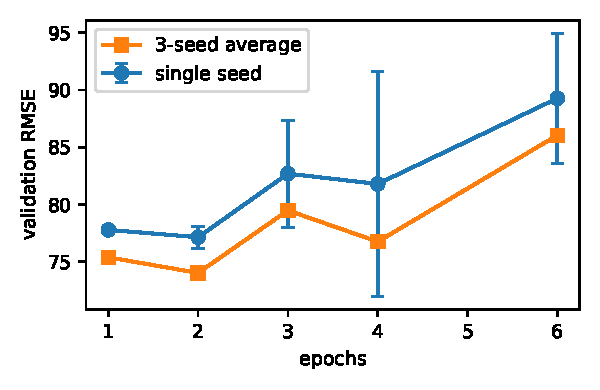
\includegraphics[width=0.45\linewidth]{../Figures/T2-3_epochs.pdf}\caption*{Fig.~T2-3 --- validation RMSE vs epochs.}\end{figure}

\subsection*{2.6 Final model, validation behaviour and limits}
\textbf{Configuration:} context 96, $d=16$, 1+1 layers, kernel 25, $k=\lfloor 2\ln L\rfloor$ (9 / 10), dropout 0.1, raw target, engineered future covariates, covariate trend start, 2 epochs.\\
\textbf{Training:} AdamW (lr $3\cdot10^{-3}$, weight decay $10^{-3}$), 10\% warm-up then cosine decay, batch 256, gradient clipping at 1.0, MSE loss, every window used (stride 1).\\
\textbf{Validation of the 3-seed average:}
\begin{itemize}
\item winter fold: RMSE 74.4, MAE 53.3, sMAPE 60.5\%;
\item recent fold: RMSE 73.6, MAE 57.1, sMAPE 66.8\%.
\end{itemize}
\begin{figure}[H]\centering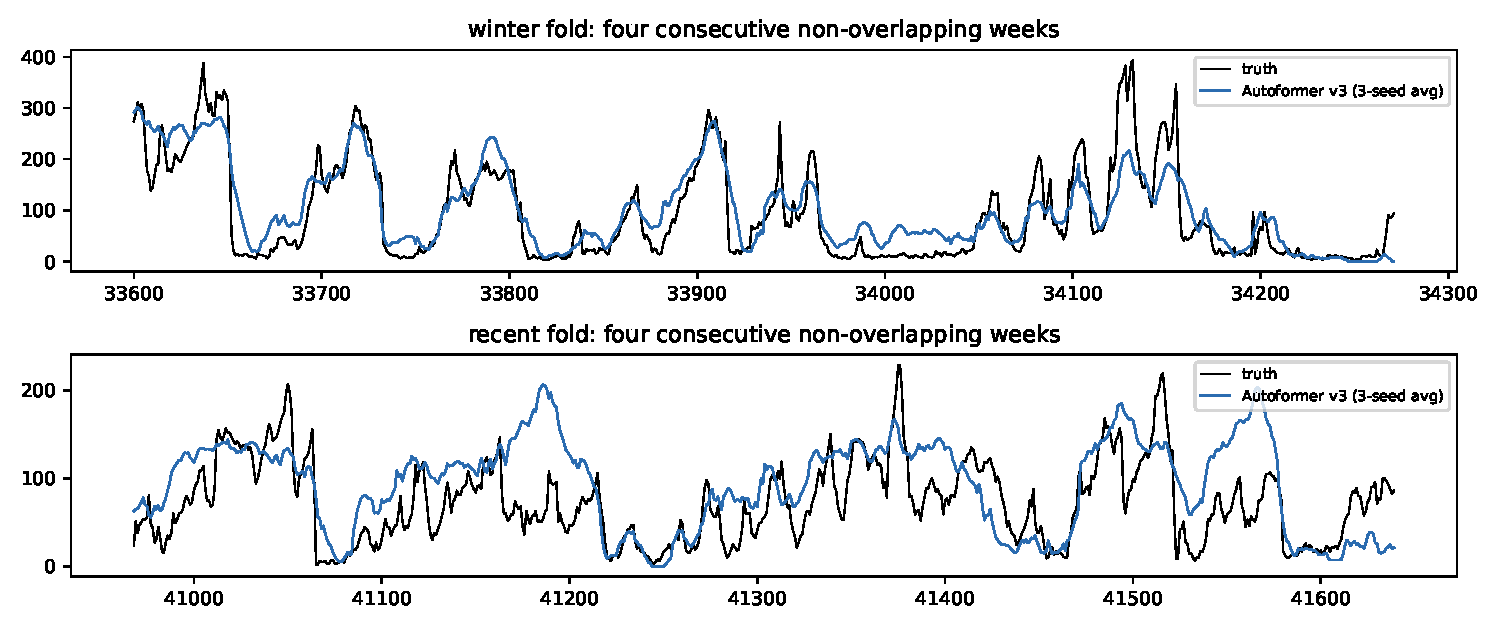
\includegraphics[width=\linewidth]{../Figures/T2-4_val_forecasts.pdf}\caption*{Fig.~T2-4 --- validation forecasts vs truth (four consecutive weeks per fold).}\end{figure}
\begin{figure}[H]\centering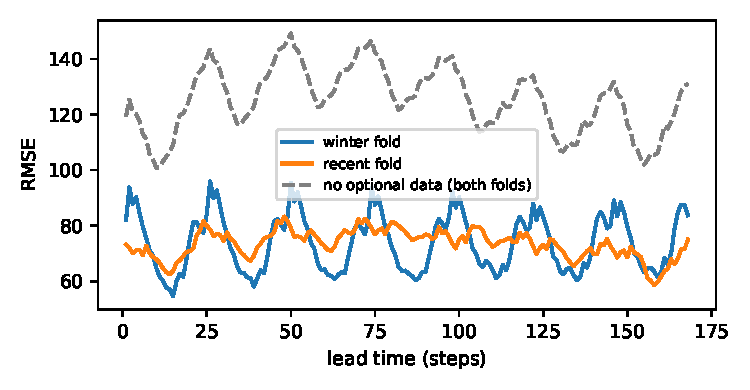
\includegraphics[width=0.5\linewidth]{../Figures/T2-5_lead_time.pdf}\caption*{Fig.~T2-5 --- RMSE by lead time.}\end{figure}
\begin{itemize}
\item \textbf{Flat error across the horizon} (Fig.~T2-5): about 73 in the first 24 steps and 75 in the last 24 (winter). The forecast is driven by the known future weather rather than by past values, so it does not drift away over the week.
\item \textbf{Weakness: the peaks.} The top 10\% of true values (above 282) carry 32\% of the squared error and are under-forecast by 103 on average, while the remaining values are over-forecast by 30. Under squared loss the model shrinks toward the conditional mean. This is also why sMAPE stays near 60\%.
\end{itemize}

\textbf{Submission.} 5 seeds, refit on the \emph{full} history for 2 epochs each, then averaged. The refit includes the newest weeks the forecast starts from. In validation, averaging seeds improved RMSE by 3 (77.1 $\to$ 74.0).
\begin{itemize}
\item $P = 5\times 9{,}159 = \mathbf{45{,}795}$ and $E = 5\times 2=\mathbf{10}$ (fixed schedule, no early stopping).
\item The size and epoch penalties together add only about 0.005 to the score.
\item Both numbers are reproducible with \texttt{python q2\_v3.py final 5}.
\end{itemize}
\begin{figure}[H]\centering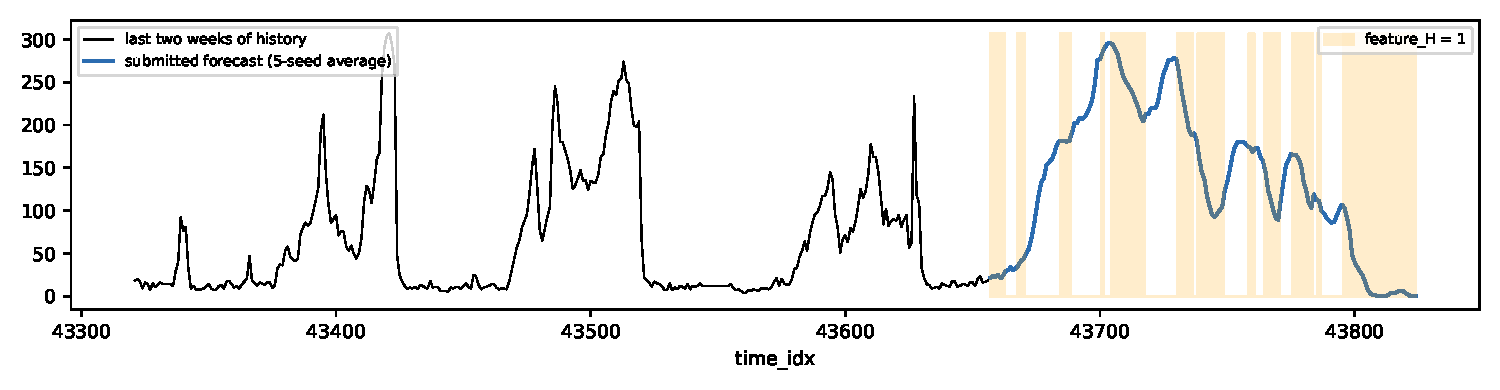
\includegraphics[width=\linewidth]{../Figures/T2-6_forecast.pdf}\caption*{Fig.~T2-6 --- submitted 168-step forecast (time\_idx 43657--43824); shaded: flag H.}\end{figure}

\textbf{Leaderboard result for this submission:} RMSE 68.34, MAE 51.54 and sMAPE 61.91\%, for a score of 68.341 with $P=45{,}795$ and $E=10$. The penalty terms add only about 0.005. The RMSE is a little better than the two-fold validation estimate (74.0); one 168-step week is a single noisy block, so I treat the leaderboard as a confirmation of the validation estimate, not as a tuning signal.

\subsection*{2.7 Reflection questions}
\begin{description}
\item[Q2.1 Auto-Correlation vs self-attention.]
\begin{itemize}
\item \emph{Where Auto-Correlation wins:} signals that repeat with a stable period, possibly several (e.g.\ a daily load cycle). Every pair at the same lag is related for the same reason, so scoring $L$ lags is better than scoring $L^2$ pairs.
\item \emph{What it discards:} content-specific links that do not repeat at a fixed lag, such as a one-off spike or a regime-dependent event. It aggregates whole shifted sequences and loses point-wise matches.
\item \emph{Drifting period:} a fixed set of lags blurs the forecast, while attention can still match individual similar points. Here the daily lag-24 structure is weak (ACF 0.40), which is why the covariates carry most of the signal.
\end{itemize}

\item[Q2.2 Moving-average trend.]
\begin{itemize}
\item \emph{What it assumes:} the trend is locally linear over the kernel, and the seasonal part averages to zero over $m$ steps.
\item \emph{At the boundaries:} endpoint replication flattens the trend near the window's end, which is exactly where the forecast starts.
\item \emph{Curvature and level shifts:} curvature is shaved off, and an abrupt level shift is smeared into a ramp of width $m$. Both matter for this heavy-tailed series.
\item \emph{Alternative:} a robust local-linear (LOESS or Hodrick--Prescott) trend. It follows curvature and the endpoint slope, but costs more computation and introduces a smoothing parameter that is harder to tune.
\end{itemize}

\item[Q2.3 Progressive vs one-shot decomposition.]
\begin{itemize}
\item \emph{What it buys:} each Auto-Correlation and FFN layer can re-introduce slow structure. Removing it after every sub-layer keeps the seasonal stream clean for the next delay scoring, and lets the decoder build the trend from learned pieces.
\item \emph{When it hurts:} if the useful signal is the level itself (as here, where the weather sets it), repeated smoothing removes it from the seasonal stream. A 24-h pollution episode is close to the kernel width (25), so it gets split between the two streams. My covariate trend start partly compensates for this.
\end{itemize}

\item[Q2.4 $k=c\log L$.]
\begin{itemize}
\item \emph{Small $k$} commits to few lags: low variance if they are right, large error if they are wrong.
\item \emph{Large $k$} hedges (like averaging) but admits noisy lags and drifts toward plain smoothing.
\item \emph{$\log L$ is convenient rather than principled:} it keeps the cost at $O(L\log L)$. Ideally $k$ should be a little larger than the number of real periodicities and their harmonics; with $L=96$, $k=9$ covers 24, 48, 72 and their neighbours.
\end{itemize}

\item[Q2.5 One-shot vs autoregressive.]
\begin{itemize}
\item \emph{Autoregressive} forecasting compounds its own errors and suffers exposure bias (it is trained on true inputs but run on its predictions). Its errors are strongly correlated along the horizon.
\item \emph{One-shot} forecasting (used here) has no feedback loop, and its error stays flat over 168 steps (Fig.~T2-5). It may produce less coherent paths.
\item \emph{When to prefer each:} autoregressive suits short horizons with smooth, low-noise dynamics. One-shot is better as the horizon and noise grow, especially when future covariates exist.
\end{itemize}

\item[Q2.6 Window normalisation.]
\begin{itemize}
\item \emph{What it destroys:} the absolute level and scale of each window.
\item \emph{Where it helps:} series whose level wanders while the shape repeats (sales with drifting demand).
\item \emph{Where it loses something essential:} when the level itself is predictable from outside, as here. "Calm, humid, southerly wind" means a high absolute value whatever the last window's mean was; stripping each window's mean throws that signal away.
\end{itemize}

\item[Q2.7 Past-only vs future-known covariates.]
\begin{itemize}
\item \emph{Where they enter:} past-only covariates belong in the encoder. Future-known ones should also enter the decoder at each forecast step, which is where the 32\% gain in S1 came from.
\item \emph{Useful only when future-known:} forecast wind speed or direction. It explains the level at the same hour but has little lagged effect beyond a day.
\item \emph{Equally useful in both:} the hour of day, which can always be computed.
\end{itemize}

\item[Q2.8 No timestamps.]
\begin{itemize}
\item \emph{What is lost:} holidays, weekdays and calendar season.
\item \emph{How to recover periodic structure:} from the index, through the autocorrelation/FFT peak (24) and the yearly position ($\approx$8,766 steps), encoded as sin/cos.
\item \emph{What this assumes:} uniform sampling (guaranteed by the handout) and that the series starts at a known phase. Otherwise only relative phase is identified.
\end{itemize}

\item[Q2.9 Structural models vs decomposition Transformers.]
\begin{itemize}
\item \emph{When structural models win:} short series, low signal-to-noise, and one dominant regular cycle. Their few parameters cannot overfit.
\item \emph{When Transformers win:} long series (tens of thousands of points), nonlinear covariate effects and several interacting regimes.
\item \emph{How to decide before training:} check the series length per parameter, the strength of the seasonal ACF peaks, and how much a linear covariate regression already explains. Here the series is long and nonlinear in the covariates, but it is noisy, so I kept the model tiny (9K parameters, 2 epochs).
\end{itemize}
\end{description}
